\section{Life History Discounting}
Brief recap: in a Leslie model setup with immutable survival vector $s = (s_1, \ldots, s_{A-1}, s_A = 0)$, initial
fecundity vector $(b_1, \ldots, b_A)$, and
Lyapunov exponent $\lambda = f(b_1, \ldots, b_A)$, we obtain that the marginal rate of substitution between additional fecundity
at age $\alpha$ and $\alpha+t$ is 
$$ \text{MRS}_{\alpha, \alpha+t} = \lambda^{-t}s_{\alpha}s_{\alpha+1}\cdots s_{\alpha+t - 1}.$$
Two factors are accounted for in this discounting regime:
\begin{enumerate}
    \item Risk - the product of the $s_a$ terms is the probability of surviving to age $\alpha+t$ given survival until $\alpha$. 
    \item Opportunity cost - accounted for in $\lambda^{-t}$, a little more difficult to rationalize beyond ``it is the only other term,''
        but it is also intuitive. The faster a population grows, the greater your opportunity cost for foregoing reproduction early is. 
\end{enumerate}
There is a continuous time analogue:
$$ \text{MRS}_{\alpha, \alpha+t} = e^{-rt}\cdot P(\text{ surv. to }\alpha+t | \text{ surv to} \alpha).
$$
If every individual in the populatio has constant risk of death, survival probability is exponential. If every individual has the same
rate parameter $\rho>0$, the population discounts exponentially. If individuals are assigned a rate parameter at birth, the aggregate
survival probability function is
$$ s(a) = \int_0^\infty e^{-\rho a} \d \gamma(a) $$
where $\gamma$ is the probability distribution of $\rho$. If $\rho$ is continuously distributed with pdf $g(\rho)$, then 
$s(a)$ is the Laplace transform of $g$, which leads to lots of nice survival and thus discounting schedules (Sozou). 

\subsection{Optimal distribution for $\rho$}
Which distribution for $\rho$ optimizes fitness? If everybody lives forever, that is the best survival function, so we need
some constraints. A natural first attempt is to ask:

\begin{center}
    \textit{Which distribution $\gamma$ optimizes fitness subject to the constraint that 
    $\mathbb{E}_{\gamma}\left[ \rho \right] = \bar{\rho}$}?
\end{center}

Regrettably, that question doesn't have an answer. Consider a two state distribution, $\rho_1$ and $\rho_2$. We pick $p_1$ and $p_2$
such that $p_1 \rho_1 + p_2\rho_2 = \bar\rho$. We have enough degrees of freedom that we can set $\rho_1 = 0$ 
and $p_1$ arbitrariy close to $1$ by making $\rho_2$ sufficiently large. That is, we can almost make almost the entire population immortal.
So trying to maximize fitness over the space of distributions for $\rho$ subject to an average $\rho$ condition is askin to trying
to maximize $f(x) = 1/x$ on $(0, 1)$. This is a little vague and hand-wavy, but it convinces me that we're trying to optimize a function
on a non-compact set, so it is not a fruitful direction. I wonder:

\begin{center}
    \textit{What is the space of feasible distributions for a risk parameter $\rho$? Is it compact? Is the mapping
    $\gamma\mapsto \lambda(\gamma) $ continuous? If so, an optimal risk parameter distribution $\gamma^*$ exists.}
\end{center}

It seems to me that I need to figure out a context in which an organism has some choice in how risk is passed onto its offspring. 
Can it take some risk away from a few to give to others? This is starting to sound like bet-hedging and egg sizes. I'll look into that.


\subsection{Discounting in Squirrel Banking}
Recall the salient details of squirrel banking: squirrels find $0, 1, $ or $2$ nuts with probabilities $p_0, p_1,$ and $p_2$ respectively. 
They bank nuts up to $\hat\beta$, consuming one each day for survival: if a squirrel has no nuts banked and finds 0 nuts, it dies. 
The squirrels in squirrel banking have survival probabilities and a fitness, so we can analyse their discounting schedule straightforwardly.
An analytic expression for the survival probability is beyond my reach. However, I can provide some intuition for how it progresses.
\begin{itemize}
    \item A squirrel's life, conditional on it still being alive, is a Markov Chain with state space $S = \left\{ 0, 1, \ldots, \hat\beta \right\}$.
    \item Start in state $0$ with probability 1. So you have initial survival probability $1 - p_0$. 
    \item The next day, you are less likely (though it is still not impossible) that you be in state 0. So you have survival probability 
        $(1-p_0)\cdot P(\text{found 0 nuts the day before})$. 
    \item The process continues: every day, you are less likely than the day before to be in state $0$, though it is still not impossible. (I think
        this relies on the assumption that the $p_2 > p_0$, the part about it being less and less likely every day). With time, the process
        coverges to its stationary distribution, at which your survival probability is the same every day. 
\end{itemize}
Numerically, it is straightforward to compute daily survival probabilities, from which we can compute
necessary appreciation of a marginal fecundity reward as we delay its receipt. In particular, if $(p_0, p_1, p_2) \approx (1, 1, 1.1)$ and
$\hat\beta = 3$, we can plot $\frac{1}{s_1s_2\cdot s_a}$, where $a$ is the horizontal axis. 
\begin{figure}[H]
    \centering
    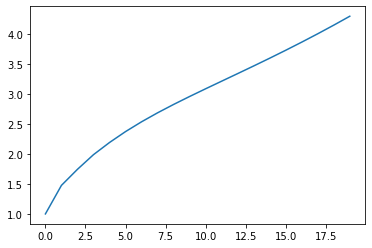
\includegraphics{inv_surv_age20}
    \caption{Inverse of survival up to age $20$ - it looks kind of flat}
\end{figure}

\begin{figure}[H]
    \centering
    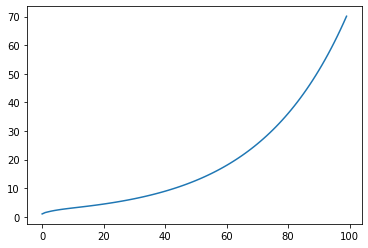
\includegraphics{inv_surv_age100}
    \caption{Inverse of survival up to age $100$ - it looks kind exponential now}
\end{figure}
This comes as no surprise. Eventually, the probability of surviving is constant, which means we are looking at exponential growth, which is what
we see in the long run. In the medium run, however, survival probability increases sufficiently quickly that we do survival's contribution to the
discounting schedule is hyperbolic, rather than exponential. I specifically picked the distribution of nuts I did so that we would get unit fitness.
We can also do this for fitness $\gtreqless1$, but I don't find much that is all that interesting. Usually the curve starts out pretty flat and then
turns exponential. 









